%% Présentation du sujet du stage [1-2 pages]

Le stagiaire, en spécialité informatique, travaille au sein du département d'ingénierie, avec pour mission d’organiser et d’optimiser les opérations d’échange d’informations entre tous les acteurs éoliens de Windeo.\\

Dans un premier temps, le stagiaire se concentrera sur la mise en place d’un système dynamique permettant d’améliorer la base de données interne, dont l'objectif est d'adapter l’espace intranet sur le site web, afin de permettre la collecte des informations et un export vers sur une base de donnée (Access, FilemakerPro ou autre) pour qu’elles constituent un récapitulatif des opérations d’intervention d’installation et de maintenance sur l’ensemble du parc éolien.\\

En ce moment, le site intranet est supporté par Wordpress (un CMS) et GoogleDoc (un outil Google), qui est figuré ci-dessous. Les clients doivent remplir plusieurs sous-formulaires (formulaire pour le mât, la turbine, etc.) sur le site de constructeur et de Windeo Green Futur, ce qui entraîne des informations redondantes et une complexité de remplissage.\\

\begin{figure}[!htbp]
  \centering
    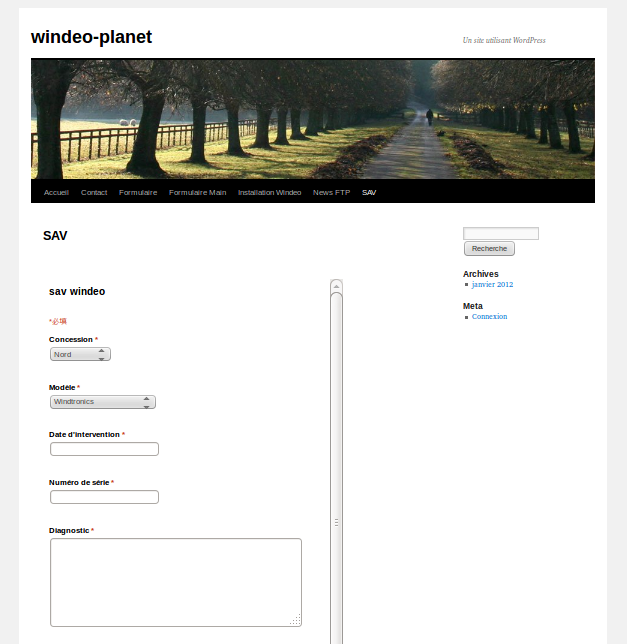
\includegraphics[scale=0.3]{images/web-old}
  \caption{Formulaire avec l'outil \texttt{GoogleDoc}}
  %\label{fig:auth}
\end{figure}

\begin{figure}[!htbp]
  \centering
    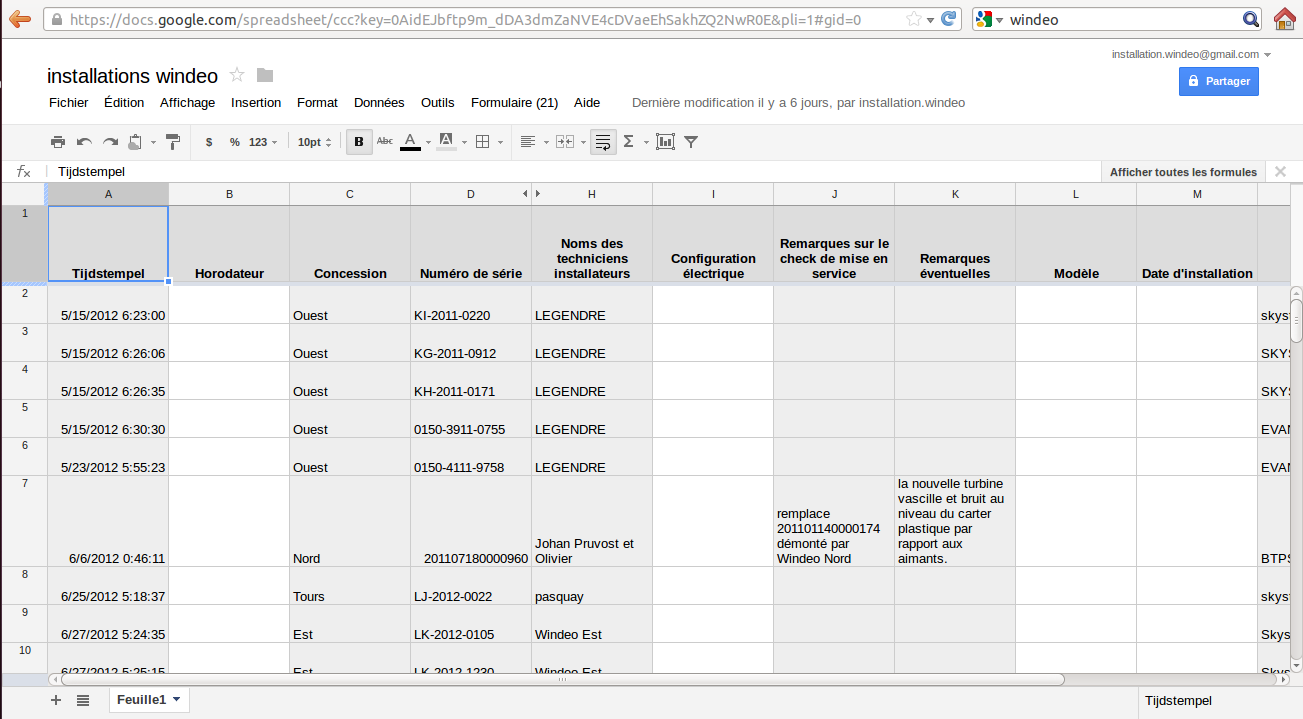
\includegraphics[scale=0.3]{images/data-old}
  \caption{Les données envoyées par \texttt{GoogleDoc}}
  %\label{fig:auth}
\end{figure}

\newpage
Une deuxième partie du stage, consistera à faciliter l’échange d’information et garantir une homogénéité des fichiers utilisés par le département d’ingénierie et les équipes techniques. La base de données repose actuellement et reposera idéalement sur un serveur File Transfert Protocol, mais tout autre système qui sera jugé intéressant par le stagiaire et l’équipe sera pris en compte. Une procédure de synchronisation des données émises et rectifiées par les participants au réseau au fur et à mesure devra être mise en place. (Procédure « Dropbox »).\\
